\documentclass[10pt,a4paper]{article}
\usepackage{fullpage}
\usepackage{amsfonts, amsmath, pifont}
\usepackage{amsthm}
\usepackage{graphicx}
\usepackage{subfig}
\usepackage{float}
\usepackage{longtable}
\usepackage{tkz-euclide}
\usepackage{titling}
\usepackage{booktabs}
\usepackage{hyperref}
\usepackage{comment}
\usepackage{tikz}
\usepackage{pgfplots}
\pgfplotsset{compat=1.13}

\setlength{\droptitle}{-7em} 
\title{CENG519 - Phase 2 Report}
\author{
  Cansu Eskici\\
  2588036}
\begin{document}
\maketitle
\section*{Introduction}
My choice of covert channel was \textit{Using options fields in TCP headers (such as timestamps) for data hiding.} 
For this purpose, I choose timestamps from TCP header options. 
This value can be used to synchronize clocks between the sender and receiver, or it can be used to measure the round-trip time of packets.
For my research, I used the following resources:
\begin{itemize}
    \item \href{https://web.mit.edu/greenie/Public/petspaper.pdf}{Covert Messaging through TCP Timestamps}
    \item \href{https://scapy.readthedocs.io/en/latest/}{Scapy Documentation}
\end{itemize}

First one is an academic paper that proposes a detailed and well structured algorithm for utilizing TCP timestamps for covert messaging. In my implementation, I did not use the same algorithm design, however it was very helpful to understand the concept of covert messaging through TCP timestamps.

The second one is Scapy documentation, I used Scapy to implement the communication between TCP client and server. 

\section*{Development}

For this project, I created a covert communication channel utilizing the least significant bits (LSBs) of the TCP timestamp option to encode and decode messages.


The sender encodes a given message into binary bits, splits it into chunks of a specified size (bits, meaning the number of LSBs to use per packet), and calculates a TCP timestamp value for each chunk based on its binary representation. 
Sender overwrites the least significant bits of the timestamp with this newly calculated value. 
This is done by masking out the LSBs and inserting the covert data, while the higher bits are randomized or incremented to mimic normal TCP behavior. 
Each modified timestamp is embedded in a TCP packet and sent to the receiver.
After all message bits are sent, the sender transmits a termination packet with a timestamp value of zero to signal the end of the covert message.
These timestamps are embedded in TCP packets and sent to a specified destination (dst\_ip and dst\_port). 


The receiver listens for TCP packets on the specified port and extracts the TCP timestamp value from each packet.
 For each received packet, it isolates the LSBs (using the same bit width as the sender) to recover the covert bits. 
 These bits are accumulated until the receiver observes a termination packet (timestamp value zero), at which point it reconstructs the original message from the collected bits.
  The receiver also pads the bitstream if necessary to ensure proper byte alignment before decoding.


\section*{Experiments}
For experimentation, the independent variables were 
\begin{itemize}
    \item \textit{Bits}, used for encoding each chunk of the message was varied across four values: 7, 8, 16, and 25.
    \item \textit{Delay}, was tested with three values: 0.01 seconds, 0.10 seconds, and 0.15 seconds.
    \item \textit{Message}, Different messages of varying lengths and content were used to test the channel's performance. The messages varied across 21, 75, 141 and 299 bytes.

\end{itemize}

The dependent variables were the average elapsed time, the capacity of the covert channel with its \%95 confidence intervals.
In order to make sure that the decoded message is correct, original message was compared with the decoded message in each experiment. 


\section*{Results}
\vspace{-2em}
\begin{figure}[H]
\centering
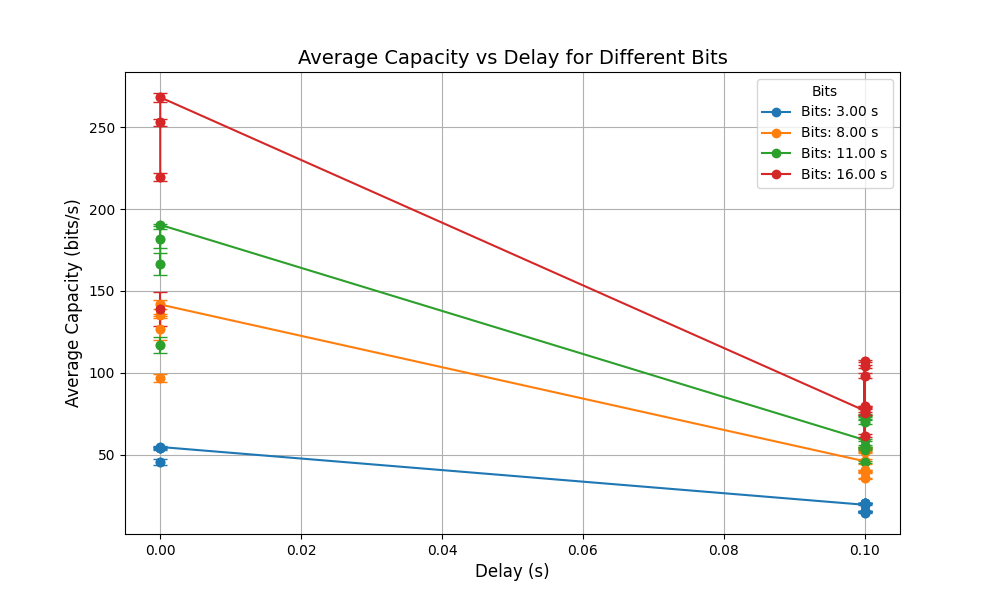
\includegraphics[width=0.8\textwidth]{capacity_vs_delay.png}
\caption{Average Capacity vs Delay}

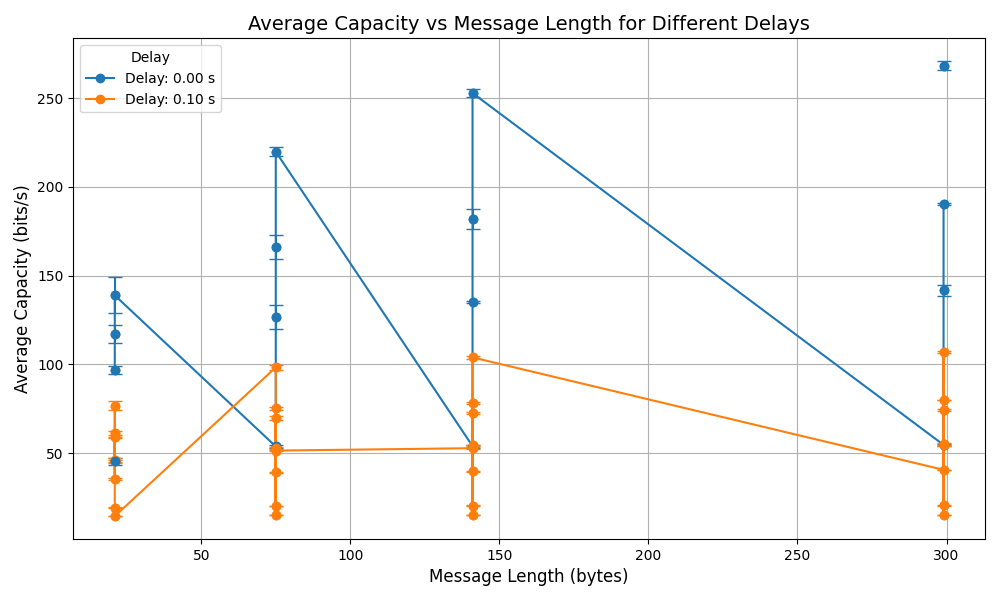
\includegraphics[width=0.7\textwidth]{capacity_vs_length.png}
\caption{Average Capacity vs Number of Bits}
\end{figure}


The experimental results clearly demonstrate the trade-offs inherent in the design of a TCP timestamp-based covert channel. The average capacity of the covert channel is primarily influenced by two factors: the delay and the number of bits used for encoding in each packet.
Increasing the delay between packets leads to a significant reduction in channel capacity. This is expected, as a longer delay directly limits the rate at which covert data can be transmitted. For example, with 7 bits per packet and a delay of 0.05 seconds, the average capacity is around 130--145 bits/s for longer messages, but drops to around 40 bits/s when the delay is increased to 0.15 seconds.
Increasing the number of bits encoded in each packet generally increases the channel capacity, up to a point. However, using a very large number of bits can introduce more padding and may make the channel more detectable or less robust, depending on network conditions. In the obtained results, higher bit-widths (e.g., 16) achieve capacities above 200 bits/s for short delays and long messages.
Longer messages tend to yield more stable and higher average capacities, as the overhead of setup and termination is amortized over more data. The confidence intervals for capacity also become narrower as message length increases, indicating more consistent performance.
Across all experiments, no corrupt messages were observed. The decoded messages always matched the original, demonstrating the reliability of the LSB-based covert channel under the tested conditions.
The complete results of the experimentation can be found the table in the next page.


\begin{table}[H]
    \centering
   \begin{tabular}{|c|c|c|c|c|c|}
    \hline
    \textbf{Bits} & \textbf{Delay (s)} & \textbf{Length (bytes)} & \textbf{Elapsed Time (s)} & \textbf{Avg Cap (bits/s)} & \textbf{Conf Interval} \\ \hline
    3 & 0.05 & 21 & 3.7131 & 45.28 & [43.37, 47.19] \\ \hline
    3 & 0.1 & 21 & 8.7054 & 19.30 & [19.07, 19.53] \\ \hline
    3 & 0.15 & 21 & 11.6185 & 14.46 & [14.28, 14.64] \\ \hline
    3 & 0.05 & 75 & 11.1668 & 53.74 & [52.66, 54.82] \\ \hline
    3 & 0.1 & 75 & 29.5414 & 20.31 & [20.25, 20.37] \\ \hline
    3 & 0.15 & 75 & 39.6026 & 15.15 & [15.09, 15.22] \\ \hline
    3 & 0.05 & 141 & 20.9134 & 53.94 & [53.14, 54.75] \\ \hline
    3 & 0.1 & 141 & 55.2073 & 20.43 & [20.39, 20.47] \\ \hline
    3 & 0.15 & 141 & 74.0659 & 15.23 & [15.18, 15.28] \\ \hline
    3 & 0.05 & 299 & 43.7885 & 54.63 & [53.99, 55.27] \\ \hline
    3 & 0.1 & 299 & 116.5072 & 20.53 & [20.44, 20.62] \\ \hline
    3 & 0.15 & 299 & 156.7475 & 15.26 & [15.23, 15.29] \\ \hline
    8 & 0.05 & 21 & 1.7384 & 96.66 & [94.39, 98.94] \\ \hline
    8 & 0.1 & 21 & 3.6628 & 45.89 & [44.47, 47.30] \\ \hline
    8 & 0.15 & 21 & 4.7371 & 35.47 & [35.10, 35.83] \\ \hline
    8 & 0.05 & 75 & 4.7400 & 126.74 & [120.09, 133.39] \\ \hline
    8 & 0.1 & 75 & 11.6741 & 51.40 & [51.10, 51.69] \\ \hline
    8 & 0.15 & 75 & 15.3037 & 39.21 & [39.00, 39.41] \\ \hline
    8 & 0.05 & 141 & 8.3356 & 135.32 & [134.66, 135.98] \\ \hline
    8 & 0.1 & 141 & 21.3806 & 52.76 & [52.35, 53.17] \\ \hline
    8 & 0.15 & 141 & 28.3113 & 39.84 & [39.55, 40.14] \\ \hline
    8 & 0.05 & 299 & 16.8828 & 141.71 & [138.74, 144.68] \\ \hline
    8 & 0.1 & 299 & 43.8644 & 54.53 & [54.25, 54.82] \\ \hline
    8 & 0.15 & 299 & 58.9632 & 40.57 & [40.53, 40.61] \\ \hline
    11 & 0.05 & 21 & 1.4358 & 117.10 & [112.19, 122.01] \\ \hline
    11 & 0.1 & 21 & 2.8537 & 58.87 & [58.39, 59.35] \\ \hline
    11 & 0.15 & 21 & 3.6916 & 45.51 & [44.90, 46.12] \\ \hline
    11 & 0.05 & 75 & 3.6108 & 166.29 & [159.54, 173.04] \\ \hline
    11 & 0.1 & 75 & 8.5973 & 69.80 & [68.64, 70.96] \\ \hline
    11 & 0.15 & 75 & 11.3469 & 52.88 & [52.50, 53.26] \\ \hline
    11 & 0.05 & 141 & 6.2000 & 182.01 & [176.45, 187.57] \\ \hline
    11 & 0.1 & 141 & 15.5720 & 72.44 & [71.76, 73.12] \\ \hline
    11 & 0.15 & 141 & 20.7125 & 54.46 & [54.18, 54.75] \\ \hline
    11 & 0.05 & 299 & 12.5631 & 190.40 & [189.67, 191.13] \\ \hline
    11 & 0.1 & 299 & 32.2634 & 74.14 & [73.57, 74.72] \\ \hline
    11 & 0.15 & 299 & 43.3510 & 55.18 & [54.79, 55.56] \\ \hline
    16 & 0.05 & 21 & 1.2120 & 138.93 & [128.78, 149.09] \\ \hline
    16 & 0.1 & 21 & 2.1883 & 76.80 & [74.44, 79.17] \\ \hline
    16 & 0.15 & 21 & 2.7382 & 61.36 & [60.46, 62.26] \\ \hline
    16 & 0.05 & 75 & 2.7289 & 219.88 & [217.39, 222.37] \\ \hline
    16 & 0.1 & 75 & 6.1037 & 98.31 & [96.88, 99.74] \\ \hline
    16 & 0.15 & 75 & 7.9808 & 75.18 & [74.39, 75.97] \\ \hline
    16 & 0.05 & 141 & 4.4596 & 252.95 & [250.72, 255.17] \\ \hline
    16 & 0.1 & 141 & 10.8522 & 103.95 & [102.96, 104.93] \\ \hline
    16 & 0.15 & 141 & 14.4513 & 78.06 & [77.55, 78.57] \\ \hline
    16 & 0.05 & 299 & 8.9140 & 268.35 & [265.73, 270.97] \\ \hline
    16 & 0.1 & 299 & 22.3323 & 107.11 & [106.44, 107.79] \\ \hline
    16 & 0.15 & 299 & 29.9707 & 79.81 & [79.65, 79.97] \\ \hline
\end{tabular}
    \caption{Average Elapsed Time, Capacity, and Confidence Intervals for Different Configurations}
    \label{tab:results}
\end{table}




\end{document}

